\section{Preliminaries}
% =========================================================================
\subsection{Complete Testing Theories}

\subsubsection*{Fault Models, Test Cases, Test Suites, and Completeness}
\label{sec:fsmfm}

We use the term \emph{signature} to denote a collection of comparable models represented 
in an arbitrary formalism. In this article, signatures represent sets of 
finite state machines
over fixed input and output alphabets, or CSP processes with finite state, represented 
by their normalised transition graphs.



Given a signature $Sig$  of models, a  \emph{fault model} ${\cal F} = (M,\le,Dom)$
specifies a \emph{reference model} $M\in Sig$, a \emph{conformance relation} 
$\le\ \subseteq Sig\times Sig$ between models, and a \emph{fault domain}
$Dom\subseteq Sig$. This terminology follows~\cite{gotzhein_fault_1996}, where
fault models were originally introduced in the context of finite state machine testing.
Note that fault domains may contain both models conforming to the reference model and
models violating the conformance relation. Note further that the reference model $M$ 
is not necessarily a member of the fault domain. For example, $M$ could be nondeterministic, while only deterministic implementation behaviours might be  considered in the fault domain.
By $F(Sig,\le)$ we denote the set of all fault models ${\cal F}$ 
defined for 
signature $Sig$ and conformance relation $\le$.

Let $\tc(Sig)$ denote the set of all \emph{test cases} applicable to
elements of $Sig$. The abstract notion of test cases defined here only requires the existence of  
 a  relation $\pass\subseteq Sig\times \tc(Sig)$. 
For
$(M,U)\in\pass$, the infix notation $M\ \pass\ U$ is used, and   interpreted as 
{\it `Model $M$ passes the test case $U$'}. 
If $(M,U)\not\in\pass$ holds, this is abbreviated by $M\ \tfail\ U$.




A \emph{test suite} $\TS \subseteq \tc(Sig)$ denotes  a set of test cases.
A model $M$ \emph{passes the test suite} $\TS$, also written as $M\ \pass\ \TS$,
if and only if $M\ \pass\ U$ for all $U\in \TS$. A test suite $\TS$ is called \emph{complete} for fault model ${\cal F} = (M,\le,Dom)$, if and only if the following properties hold.
\begin{enumerate}
\item If a member $M'$ of the fault domain  conforms to the reference model $M$, 
it passes the test suite, that is,
$$
\forall M'\in Dom: M'\le M \Rightarrow M'\ \pass\ \TS
$$
This property is usually called \emph{soundness} of the test suite.

\item If a member of the fault domain passes the test suite, it conforms to the reference model, that is,
$$
\forall M'\in Dom: M'\ \pass\ \TS \Rightarrow M'\le M
$$
This property is usually called \emph{exhaustiveness}.
\end{enumerate}
A test suite $\TS$ is \emph{finite} if it contains finitely many test cases and every test
case $U\in\TS$ is finite in the sense that it terminates after a finite number of steps.
It is trivial to see that, if $\TS$ is complete  for   ${\cal F} = (M,\le,Dom)$
and $Dom'\subseteq Dom$, then $\TS$ is also complete for ${\cal F}' = (M,\le,Dom')$.



%A \emph{complete testing theory} is a mapping (again denoted by $\TS$)
%$\TS : F \fun \Pwr(\tc(Sig))$
%from a set $F$ of fault models to test suites,  such that  the test suites
%$\TS({\cal F})$ are complete
%for all fault models  ${\cal F} \in F$. A testing theory 
%$\TS : F \fun \Pwr(\tc(Sig))$ is
%\emph{finite} if and only if 
%$\TS({\cal F})$ is a finite test suite for all ${\cal F}\in F$.
%In analogy, sound and exhaustive testing theories are defined.


% ============================================================================
\subsection{Translation of Testing Theories}
\label{sec:transltt}

Let $Sig_1$ and $Sig_2$ be two signatures with conformance relations $\le_1$ and $\le_2$,
and test case relations $\pass_1$ and $\pass_2$, respectively. 
A function $T:\underline{Sig_1} \fun Sig_2$ defined on a sub-domain $\underline{Sig_1} \subseteq Sig_1$  
 is called
a \emph{model map}, and a function $T^*:\tc(Sig_2) \fun \tc(Sig_1)$ is called a \emph{test case map}. Note that models and test cases are mapped in opposite directions 
(see Fig.~\ref{fig:satisfaction-relation}).
The pair $(T,T^*)$ fulfils the \emph{satisfaction condition} if and only if the following conditions {\bf SC1} and {\bf SC2} are fulfilled.
\begin{description}
\item[\bf SC1] The model map is compatible with the conformance relations under consideration, in the sense that
$$
\forall {\cal S},{\cal S}'\in \underline{Sig_1}: {\cal S}' \le_1 {\cal S} \Leftrightarrow 
T({\cal S}') \le_2 T({\cal S}),
$$
so   the left-hand side diagram   in Fig.~\ref{fig:satisfaction-relation} commutes due to the fact that
$T;\le_2 = \le_1;T$.\footnote{Operator ``;'' denotes the relational composition defined for
functions or relations $f\subseteq A\times B$, $g\subseteq B\times C$ by 
$f;g = \{(a,c)\in A\times C~|~\exists b\in B: (a,b)\in f \wedge (b,c)\in g\}$.
Note that $f;g$ is evaluated from left to right (like composition of code fragments), 
as opposed to right-to-left evaluation which is usually denoted by $g\circ f$.}

\item[\bf SC2] Model map and test case map preserve the $\pass$-relationship in the sense that
$$
\forall {\cal S}\in \underline{Sig_1}, U \in\tc(Sig_2): T({\cal S})\ \pass_2\ U \Leftrightarrow {\cal S}\ \pass_1\ T^*(U), 
$$
so the right-hand side diagram   in Fig.~\ref{fig:satisfaction-relation} commutes, due to the fact that
$\pass_1 = T;\pass_2;T^*$. 
\end{description}

% ............................................................................
\begin{figure}
\centering
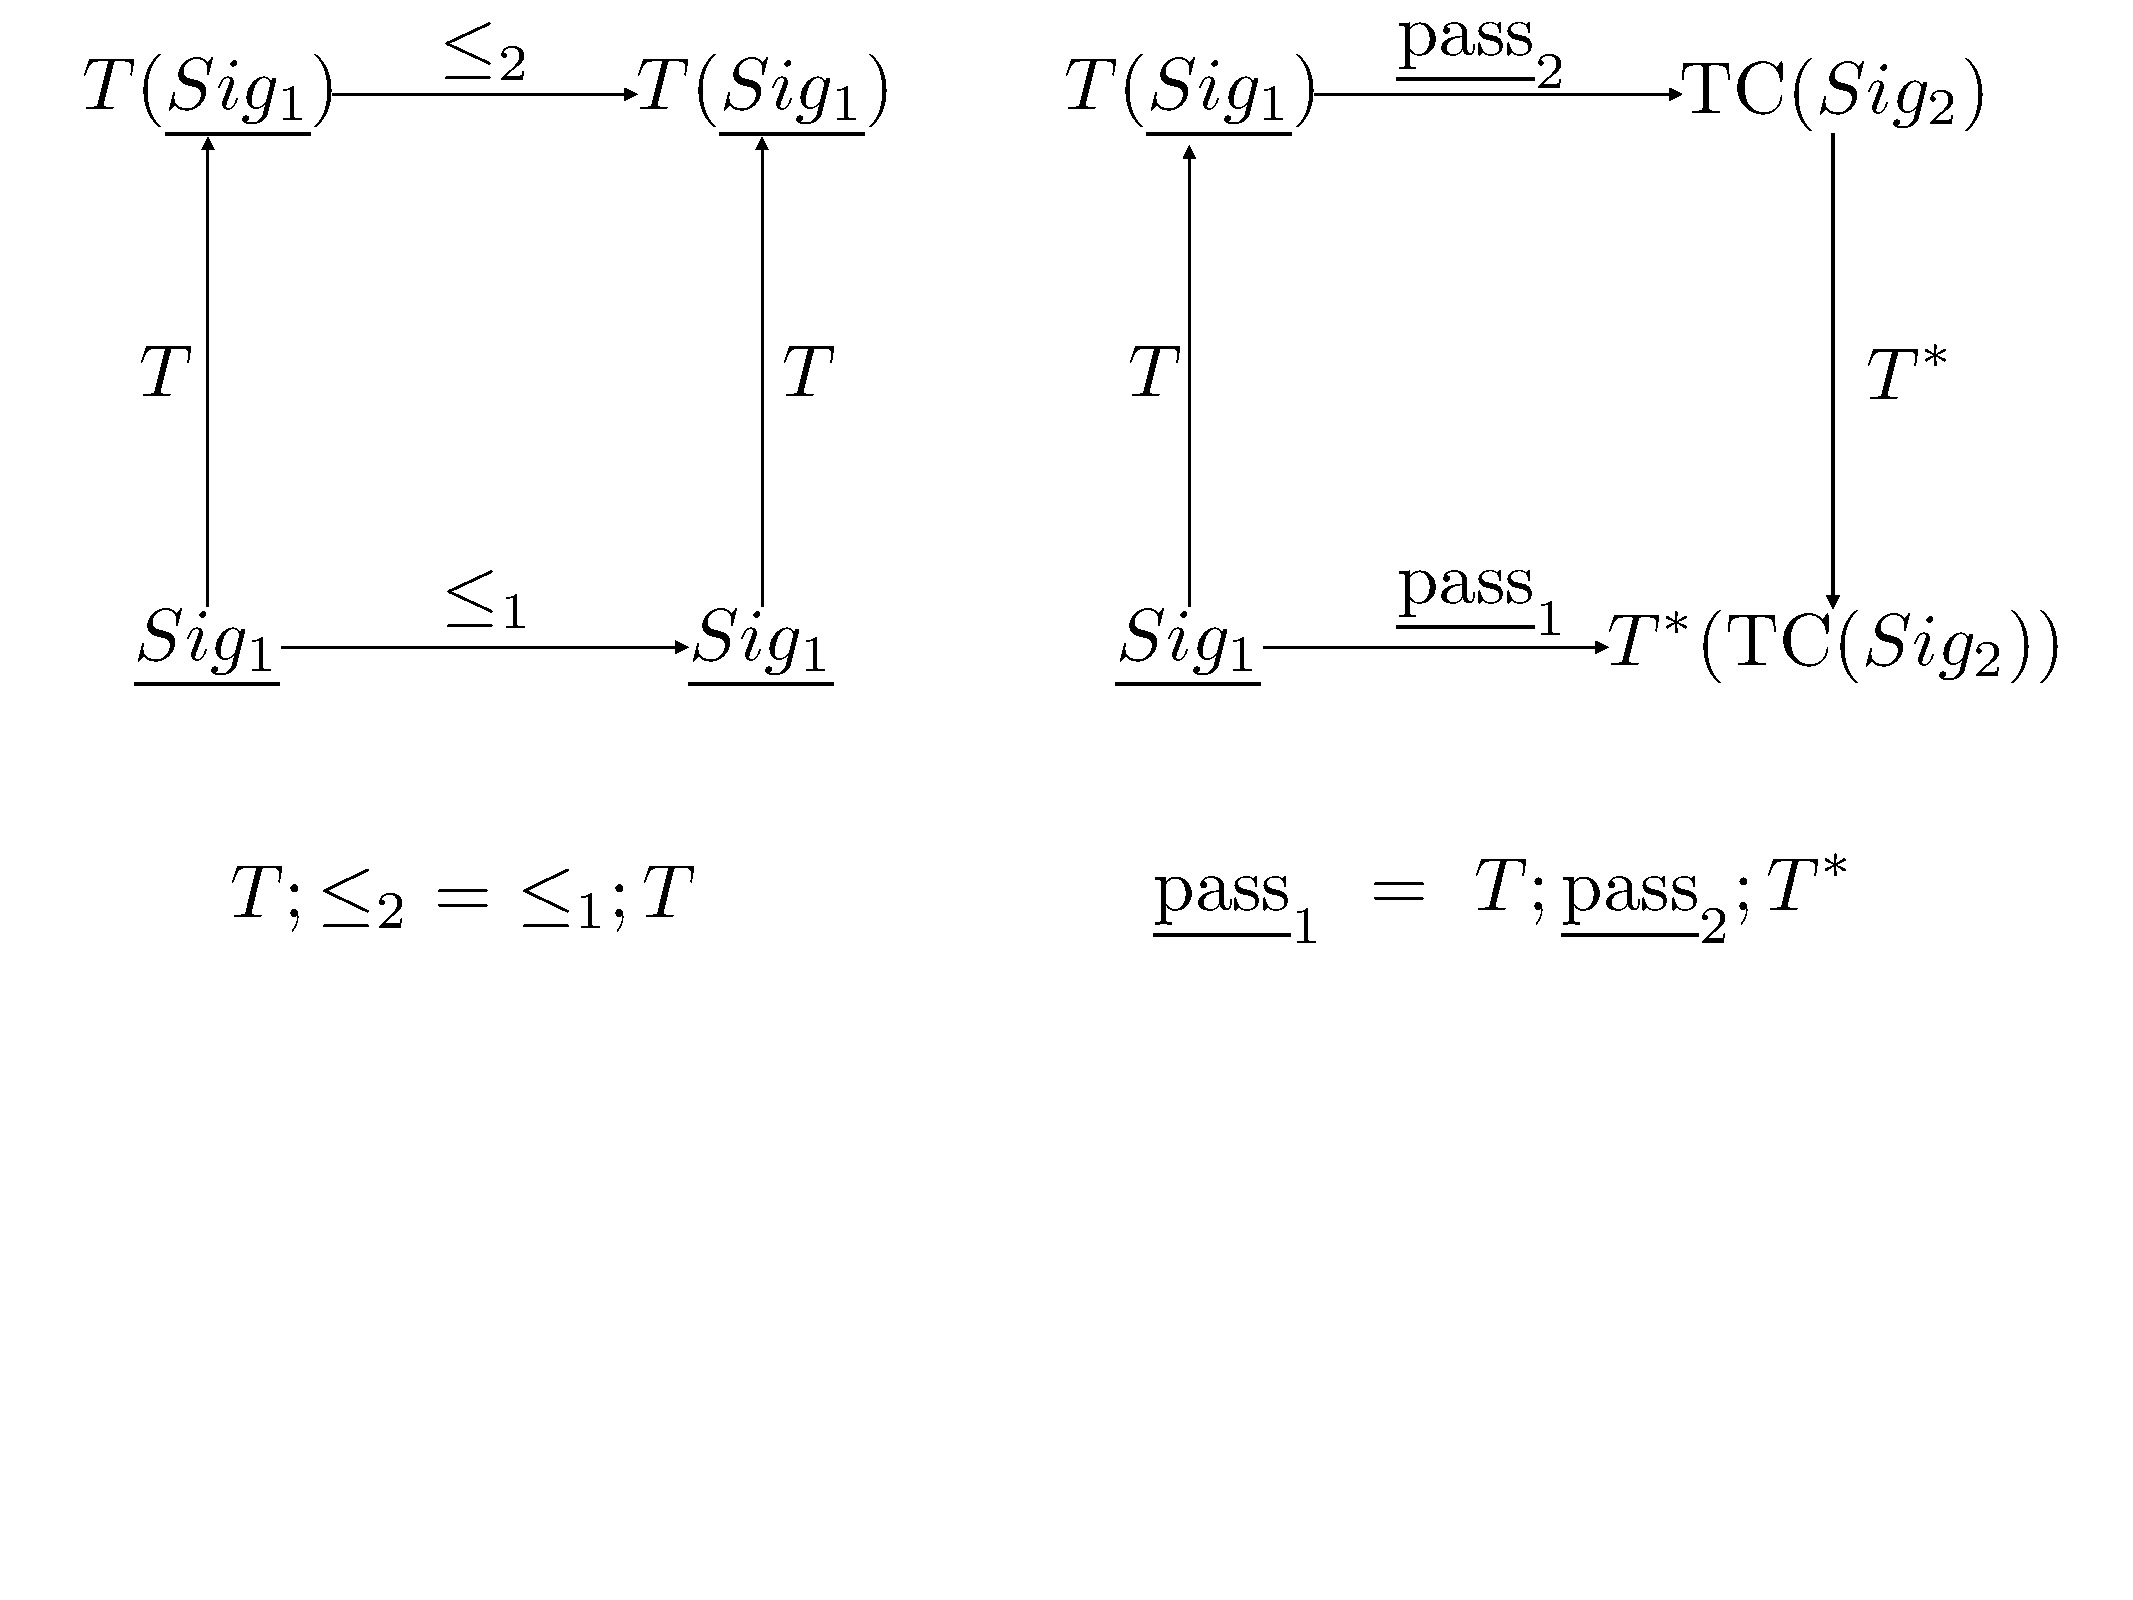
\includegraphics[width=0.6\textwidth]{satisfaction-condition.pdf}
\vspace*{-20mm}
 \caption{Commuting diagrams reflecting the satisfaction condition.}
 \label{fig:satisfaction-relation}
 \end{figure}
% .............................................................................

 

% ============================================================================

 The following theorem is a direct consequence of~\cite[Theorem~2.1]{Huang2017}.

\begin{theorem}\label{th:theorytranslation}
With the notation introduced above, let  $(T,T^*)$ fulfil the satisfaction condition.
Suppose that $\TS_2 \subseteq TC(Sig_2)$ is a complete test suite
for fault model ${\cal F}_2 = ({\cal S}_2,\le_2,Dom_2)$. Define fault model ${\cal F}_1$ on 
$\underline{Sig}_1$ by
$$
{\cal F}_1 = ({\cal S}_1,\le_1,Dom_1),\ \text{such that}\
T({\cal S}_1)  =  {\cal S}_2\ \text{and}\
Dom_1  =  \{ {\cal S}~|~T({\cal S})\in Dom_2 \}.
$$
Then
$$
\TS_1 = T^*(\TS_2)
$$
is a complete test suite with respect to fault model ${\cal F}_1$.
\xbox
\end{theorem}

 
 


% =========================================================================
\subsection{CSP and Refinement}

% -------------------------------------------------------------------------
\subsubsection*{Normalised Transition Graphs}

As shown in~\cite{Roscoe:1994:CME:197600}, any finite-state CSP process $P$ can be represented by a \emph{normalised transition graph} 
$$
G(P) = ( N, \ii n, \Sigma, t : N\times\Sigma \pfun N, a : N \fun \mathbb{P}\mathbb{P}(\Sigma)),
$$
with nodes $N$, initial node $\ii n\in N$, and process alphabet $\Sigma$. The partial \emph{transition function} $t$ maps a node $n$ and an event $e\in\Sigma$ to its successor node $t(n,e)$, if and only if $(n,e)$ are in the domain of $t$. Normalisation of $G(P)$ is reflected 
by the fact that $t$ is a function. The total function $a$ maps each node to its set of \emph{minimal acceptances}: 
if $n\in N$ corresponds to a deterministic process state of $P$, $ac(n)$ contains a single acceptance $A\subseteq \Sigma$, and every $e\in A$ is in one-one-correspondence with a transition $t(n,e)$. If $n$ corresponds to a nondeterministic process state, $ac(n)$ contains at least two acceptances $A_1, A_2, \dots, A_k$. This reflects the fact that in a nondeterministic state, $P$ must accept all events of one acceptance 
$A_i, i \in \{ 1,\dots,k\}$, but may refuse all events $e$ from 
$A_j \setminus A_i, j\neq i$. 

Each well-defined transition graph $G(P)$ fulfils the following condition. The union of all minimal acceptances in each node corresponds to the set of events labelling its outgoing transitions.
\begin{equation}
\label{eq:wellformedg}
\forall n\in N: (n,e)\in\dom~t \Leftrightarrow e\in\bigcup ac(n)
\end{equation}
In this condition, $\dom~t$ denotes the domain of function $t$. 

By construction, normalised transition graphs reflect the failures semantics of finite-state CSP processes: 
the traces $s$ of a process are exactly the paths through the transition graph, 
starting at $\ii n$. The maximal refusals in each process state $P/s$
 are the complements of 
the minimal acceptances of the node $n$ 
corresponding to $P/s$. As a consequences, all failures 
of $P$ are represented by some $(s,R)$, where $s$ is an initialised path through the transition graph and $R\subseteq (\Sigma-A)$ for some minimal acceptance $A\in ac(n)$, 
such that $n$ is the node corresponding to $P/s$. 

\begin{example}\label{ex:a}
Consider CSP process 
\begin{eqnarray*}
P & = & a \then (Q\intchoice R)
\\
Q & = & a \then P \extchoice c \then P
\\
R & = & b \then P \extchoice c \then R
\end{eqnarray*}
Its transition graph $G(P)$ is shown in Fig.~\ref{fig:tga}. Process state $P$ is represented there as Node\_0, with $\{ a\}$ as the only acceptance, since event $a$ can never be refused, and no other events are accepted. Having engaged into $a$, the transition emanating from Node\_0 leads to Node\_2 representing  the process state 
$P/a = Q\intchoice R$. The internal choice operator induces several acceptance sets derived from $Q$ and $R$. Since these processes accept their initial events with external choice, 
process $Q\intchoice R$ induces just two minimal acceptance sets $\{a,c\} = [Q]^0$ and
$\{b,c\} = [R]^0$. Note that event $c$ can never be refused, since it is a member of all minimal acceptances. 

Having engaged into $c$, the next process state is represented by Node\_1. Due to normalisation, there was only a single transition satisfying 
$t(\text{Node\_2},c) = \text{Node\_1}$. This transition, however, can have been caused 
by either $Q$ or $R$ engaging into $c$, so Node\_1 corresponds to process state
$Q/c \intchoice R/c = P \intchoice R$. This is reflected by the two minimal acceptances
labelling Node\_1. 
\xbox
\end{example}


% .....................................................................................
 \begin{figure}
 %%\hspace*{-40mm}
 \begin{center}
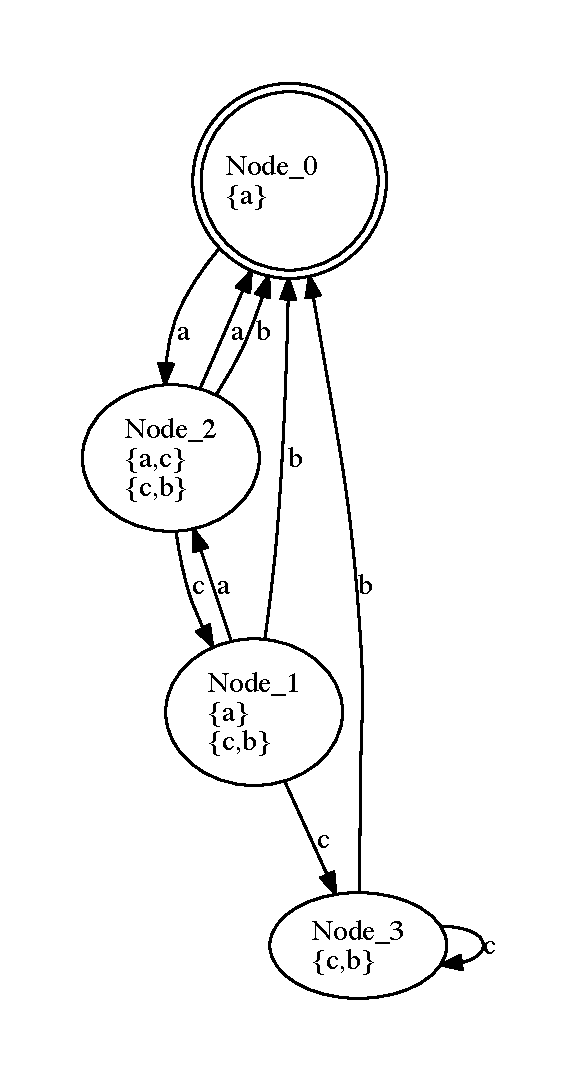
\includegraphics[width=.5\textwidth]{q0.pdf}
\end{center}
%%\vspace*{-10mm}
\caption{Normalised transition graph of CSP process $P$ from Example~\ref{ex:a}.}
 \label{fig:tga}
 \end{figure}
% ....................................................................................... 



% =========================================================================
\subsection{Finite State Machines}


To make this paper sufficiently self-contained, we introduce definitions, notation, and facts
about 
finite state machines (FSMs) that have been originally described in contributions on FSM testing, such as~\cite{petrenko_testing_2011,DBLP:conf/hase/PetrenkoY14,hierons_testing_2004}.

% -----------------------------------------------------------------------------------
A \emph{Finite State Machine (FSM)} is  a tuple
 $M=(Q, \ii{q}, \Sigma_I, \Sigma_O,  h)$   with state space $Q$, input alphabet $\Sigma_I$, 
 output alphabet $\Sigma_O$, where $Q,\Sigma_I,\Sigma_O$ are finite and nonempty sets. $\ii{q}\in Q$ denotes the initial state. 
$h\subseteq Q\times \Sigma_I \times \Sigma_O\times Q$ is the  transition relation,  $(q,x,y,q')\in h$ if and only if there is a transition from $q$ to $q'$ with input $x$ and output $y$. 
We use  both set notation $(q,x,y,q')\in h$ and Boolean notation $h(q,x,y,q')$ for specifying
that $(q,x,y,q')$ is a transition in $h$.
We call $x$ a \emph{defined} input in state $q$, if there is a transition from $q$  with input $x$. 
If every input of $\Sigma_I$ is defined in every state, $M$ is \emph{completely specified}.
If in every state $q$ and for every output $y\in\Sigma_O$, and input $x$ and a post-state 
$q'$ satisfying $h(q,x,y,q')$ exists, the FSM is called \emph{output complete}.


FSM $M$ is called a \emph{deterministic FSM (DFSM)}, if for any state $q$ and defined input $x$,
$h(q,x,y,q') \wedge h(q,x,y',q'')$ implies $(y,q') = (y',q'')$. Intuitively speaking, a specific 
input applied to a specific state uniquely determines both post-state and associated output.
If $M$ is not deterministic, it is called a \emph{nondeterministic FSM (NFSM)}.  
If there is no emanating transition for $q\in Q$, this state is called a \emph{deadlock state}, and
\emph{$M$ terminates in $q$}. The set of deadlock states is denoted by $\deadlock(Q)\subseteq Q$. 
The set of states that do not deadlock is denoted by 
$\DF(Q) = \{ q\in Q~|~\exists (q',x,y,q'')\in h: q' = q \}$.

 
The transition relation $h$ can be extended in a natural way to input traces:  
let $\overline{x}$ be an input trace and $\overline{y}$ an output trace. Then 
$(q,\overline{x},\overline{y},q')\in h$, if and only if there is a transition sequence
from $q$ to $q'$ with input trace $\overline{x}$ and output trace $\overline{y}$. 
If $q$ is the initial state $\ii{q}$, such a transition sequence is called an \emph{execution} of $M$. Executions are written in the notation 
$$
q_0 \xrightarrow{x_1/y_1} q_1 \xrightarrow{x_2/y_2} \dots \xrightarrow{x_{k}/y_{k}} q_{k}
$$ 
with $q_0 = \ii{q}$, $h(q_{i-1},x_i,y_i,q_{i})$ for $i = 1,\dots,k$, and
$\overline{x} = x_1\dots x_k$ and $\overline{y} = y_1\dots y_k$.

The empty trace is denoted by $\varepsilon$, and
$(q,\varepsilon,\varepsilon,q)\in h$, for any state $q$.
A \emph{language}  of an FSM $M$  is the set consisting of all possible input/output
traces in $M$; we use notation
 $L_M(q)=\{\overline{x}/\overline{y}~|~\exists q'\in Q: h(q,\overline{x},\overline{y},q')\}$ for $q\in Q$, and  $L(M)=L_M(\ii{q})$.
By $\fsm(\Sigma_I,\Sigma_O)$ we denote the set of all FSMs with input alphabet $\Sigma_I$ and
output alphabet $\Sigma_O$.

An FSM $M$ is called \emph{observable} if in every state $q$, every existing post-state $q'$ is uniquely determined by the I/O pair $x/y$ satisfying $h(q,x,y,q')$. For
observable state machines, the partial function
$$
h_1 : Q\times\Sigma_I\times \Sigma_O \pfun Q;\    
h_1(q,x,y) = q' \Leftrightarrow h(q,x,y,q')
$$
is well-defined. Deterministic FSMs are always observable.

% -----------------------------------------------------------------------------------
Two FSM $M_1, M_2$ are \emph{I/O-equivalent ($M_1\sim M_2$)} if and only if their languages coincide, i.e.~$L(M_1) = L(M_2)$. FSM $M_1$ is a \emph{reduction of $M_2$ ($M_1 \preceq M_2$)},
if and only if $L(M_1) \subseteq L(M_2)$. I/O-equivalence is also called 
\emph{trace equivalence} by some authors, see, e.g.~\cite{luo_test_1994}.
